\definecolor{mygreen}{rgb}{0,0.6,0}
\definecolor{mygray}{rgb}{0.5,0.5,0.5}
\definecolor{mymauve}{rgb}{0.58,0,0.82}

%%%%%%%%%%%%%%%%%%%%%%%%%%%%%%%%%%%%%%%%%%%%%%%%%%%%%%%%%%%%%%%%%%%%%%%%%%%%%
% parámetros para configurar el formato del código en los entornos lstlisting
%%%%%%%%%%%%%%%%%%%%%%%%%%%%%%%%%%%%%%%%%%%%%%%%%%%%%%%%%%%%%%%%%%%%%%%%%%%%%
\lstset{ %
  backgroundcolor=\color{white},   % choose the background color; you must add \usepackage{color} or \usepackage{xcolor}
  basicstyle=\footnotesize,        % the size of the fonts that are used for the code
  breakatwhitespace=false,         % sets if automatic breaks should only happen at whitespace
  breaklines=true,                 % sets automatic line breaking
  captionpos=b,                    % sets the caption-position to bottom
  commentstyle=\color{mygreen},    % comment style
  deletekeywords={...},            % if you want to delete keywords from the given language
  escapeinside={(*@}{@*)},          % if you want to add LaTeX within your code
  %extendedchars=true,              % lets you use non-ASCII characters; for 8-bits encodings only, does not work with UTF-8
  %frame=single,	                % adds a frame around the code
  keepspaces=true,                 % keeps spaces in text, useful for keeping indentation of code (possibly needs columns=flexible)
  keywordstyle=\color{blue},       % keyword style
  language=[ANSI]C,                % the language of the code
  %otherkeywords={*,...},           % if you want to add more keywords to the set
  numbers=left,                    % where to put the line-numbers; possible values are (none, left, right)
  numbersep=5pt,                   % how far the line-numbers are from the code
  numberstyle=\tiny\color{mygray}, % the style that is used for the line-numbers
  rulecolor=\color{black},         % if not set, the frame-color may be changed on line-breaks within not-black text (e.g. comments (green here))
  showspaces=false,                % show spaces everywhere adding particular underscores; it overrides 'showstringspaces'
  showstringspaces=false,          % underline spaces within strings only
  showtabs=false,                  % show tabs within strings adding particular underscores
  stepnumber=1,                    % the step between two line-numbers. If it's 1, each line will be numbered
  stringstyle=\color{mymauve},     % string literal style
  tabsize=2,	                   % sets default tabsize to 2 spaces
  title=\lstname,                  % show the filename of files included with \lstinputlisting; also try caption instead of title
  morecomment=[s]{/*}{*/}
}

\chapter{Diseño e implementación} % Main chapter title
\label{Chapter3} % Change X to a consecutive number; for referencing this chapter elsewhere, use \ref{ChapterX}

En este capítulo se describen los aspectos más relevantes del diseño e implementación de la plataforma. Inicialmente se presenta su arquitectura en donde se describen sus componentes e interacciones. Luego se describe el proceso de despliegue de la infraestructura de soporte, tanto en ambiente local como en ambiente de producción. Posteriormente se enfatiza la tarea de etiquetado de datos, incluyendo los problemas y soluciones enfrentados. Finalmente se presenta el entrenamiento de los modelos, seguido del despliegue e integración con el resto de la plataforma.

%----------------------------------------------------------------------------------------
%	SECTION 1
%----------------------------------------------------------------------------------------
\section{Arquitectura de la plataforma}
\label{sec:arquitectura}

El objetivo principal de este trabajo fue brindar una introducción a un sistema completo de monitoreo y detección de la plaga del picudo rojo mediante imágenes aéreas generadas por drones y/o aviones. El enfoque se basó en el módulo de VPC, donde se destacan los hitos que fueron necesarios ejecutar dentro de la IM para llevar a cabo el trabajo. Entre estos hitos se encuentra el proceso de gestión de datos, la correcta administración de los modelos de VPC y la infraestructura que soporta estos procesos. Para ello, se planteó la plataforma de la figura \ref{fig:plataforma}. Esta plataforma se basa en un enfoque modular, donde cada componente desempeña un papel específico en el proceso de detección y monitoreo de la infección.

\begin{figure}[H]
  \centering
  \includegraphics[scale=0.06]{./Figures/arquitectura-solución.png}
  \caption{Diagrama de arquitectura del sistema de monitoreo.}
  \label{fig:plataforma}
\end{figure}

El sistema se organiza en dos ecosistemas diferenciados: uno constituido por herramientas externas a la infraestructura de la IM, y otro integrado por herramientas internas.

El ecosistema externo se encarga de las interaccione con plataformas de servicios externos, como lo es Google Maps, en donde al momento de realizar el trabajo se encontraba la información relevada por el servicio de arbolado. En un futuro, esta información estaría integrada a sistemas dentro de la IM, como lo es QGIS \citep{wikipedia_qgis_2025}.

Por otra parte, en el ecosistema interno se incluyen todas las herramientas necesarias para llevar a cabo un proyecto de VPC, encapsuladas dentro de la infraestructura de la IM. Este ecosistema se basa en software de código abierto y se divide en varios módulos, lo que aumenta la sustituibilidad de piezas de software (atributo comúnmente conocido intercambiabilidad en patrones de arquitecturas de software). La comunicación se basa en protocolos ligeros como REST \citep{wikipedia_protocolo_2024}, que generan un bajo acoplamiento y una alta cohesión entre módulos. Esta plataforma cuenta también con varios módulos definidos para procesos auxiliares como la seguridad, los respaldos y la gestión de la configuración.

El módulo de seguridad permite la administración de usuarios y permisos. Esto garantiza que solo los usuarios autorizados tengan acceso a la información sensible. Este módulo se basa en el protocolo LDAP, que favorece una gestión centralizada de autenticación y autorización. Adicionalmente, el módulo puede ser sustituido por el software utilizado en la IM (WSO2 \citep{wso2_deliver_nodate}) o directamente interactuar con este (WSO2 puede comunicarse mediante el protocolo LDAP).

El módulo de respaldo de datos cerciora que los datos estén siempre disponibles y que se puedan recuperar en caso de pérdida. Gestiona procesos de respaldo y recuperación de datos, lo que mitiga riesgos asociados a la pérdida de información. Al ser un módulo independiente, puede ser sustituido por otro software de respaldo, como por ejemplo: Restic \citep{restic_restic_nodate} o Bacula \citep{bacula_documentation_nodate}.

El módulo gestor de datos es el encargado de almacenar los metadatos de las imágenes y los resultados de los modelos. Está conformado por una base de datos orientada a documentos, que permite almacenar varios tipos de datos (explicado en la sección \ref{sec:gestionRepoDatos}). Esta forma de almacenamiento, que mejora la eficiencia, facilita la gestión de grandes volúmenes de información. Asimismo, esta estructura también soluciona el desafío guardar las etiquetas generadas por los usuarios en el proceso de etiquetado de datos.

El módulo de etiquetado de datos permite ejecutar el proceso de etiquetado de imágenes y se comunica tanto con el módulo de seguridad para el manejo de diferentes niveles de información, así como con el módulo gestor de datos para almacenar las etiquetas generadas por los usuarios. Este módulo intenta estar bajamente acoplado en todo momento, por lo que la integración con repositorios de datos y proveedores de identidad es esencial para su funcionamiento.

El módulo de calidad de datos se ocupa de realizar un análisis cualitativo de los datos, lo que mejora la eficiencia de los modelos al utilizar datos de alta calidad. Este módulo permite que un equipo de control de calidad pueda analizar y generar informes específicos sobre los datos, lo que habilita una traza y evolución de lás imágenes, esencial en proyectos de VPC donde la variable temporal afecta el resultado de las predicciones, como lo es este trabajo.

El módulo de información georreferenciada permite resolver la ubicación de los elementos de interés. Esto concede que los datos estén correctamente posicionados para así emparejar las predicciones de los modelos y las coordenadas reales. Además, este módulo brinda información con mayor granularidad y un historial de los elementos, como lo son las palmeras y sus antecedentes de infección.

El módulo de repositorio de objetos es el responsable del almacenamiento y gestión de las imágenes, en este caso las generadas por drones y aviones. Este módulo administra grandes volúmenes de diferentes tipos de datos y garantiza la disponibilidad continua de esta información mediante APIs. Para esta tarea, usualmente se utilizan sistemas de almacenamiento de objetos como Amazon S3 \citep{amazon_web_services_aws_nodate} o algún otro proveedor de nube.

El módulo de aplicaciones web se encarga de gestionar la interfaz de usuarios, lo que les permite interactuar con el sistema y acceder a la información de manera sencilla. Interactúa con el sistema de información georreferenciada y muestra información sobre los elementos de interés, como las palmeras y su estado de actual de infección. También permite ingresar nueva información al sistema como nuevos focos de detección de la plaga. Esto asegura que el sistema esté actualizado en todo momento y facilita a los usuarios la visualización e identificación de estos focos.

El módulo mini-apps centraliza aplicaciones utilizadas en varias tareas, como la actualización, migración y generación de datos que usualmente son insumos para los procesos de entrenamiento. Este módulo realiza tareas específicas que no están directamente relacionadas con el proceso de detección, pero que son necesarias para el correcto funcionamiento del sistema. Un ejemplo de esto es la aplicación que efectúa \textit{web scrapping} del sistema de información geográfica de la IM, para descargar las imágenes de los vuelos allí publicadas y guardarlas en el repositorio de imágenes.

Finalmente, el módulo de IA se encarga de cumplir con los procesos asociados al entrenamiento y despliegue de los modelos. Tiene el objetivo de manejar sus el ciclos de vida, desde su desarrollo hasta su despliegue en producción. Incluye la administración de experimentos y expone una API para la interacción con otros elementos del sistema, como las aplicaciones web o las mini-apps.


La interacción entre estos componentes permite que el sistema funcione de manera eficiente y escalable. Cada módulo se encarga de una tarea específica, lo que se alinea con SRP (sigla del inglés \textit{Single Responsibility Principle} \citep{soni_software_2024}). Esto posibilita una fácil sustitución y mejora continua del sistema. Este tipo de arquitecturas también favorece la integración de nuevas funcionalidades y la adaptación a cambios en los requisitos de la solución. Si bien el enfoque principal del trabajo fue sobre el módulo de IA, se utilizaron herramientas de soporte que satisfacen este enfoque modular, como las que se describen en la siguiente sección.

%----------------------------------------------------------------------------------------
%	SECTION 2
%----------------------------------------------------------------------------------------

\section{Despliegue de la infraestructura de soporte}
\label{sec:despliegue_infraestructura}

El despliegue de la infraestructura de soporte se llevó a cabo en dos ambientes, uno local y otro de producción.

El entorno local se utilizó para el desarrollo y la ejecución de pruebas preliminares, mientras que el de producción, que intenta replicar la infraestructura operativa de la IM, se destinó al despliegue final del sistema.

En este contexto, el dominio local se configuró para emular el entorno de producción mediante la adopción de herramientas idénticas o análogas, tal como se ilustra en la figura \ref{fig:infra-desarrollo}.

\begin{figure}[htpb]
  \centering
  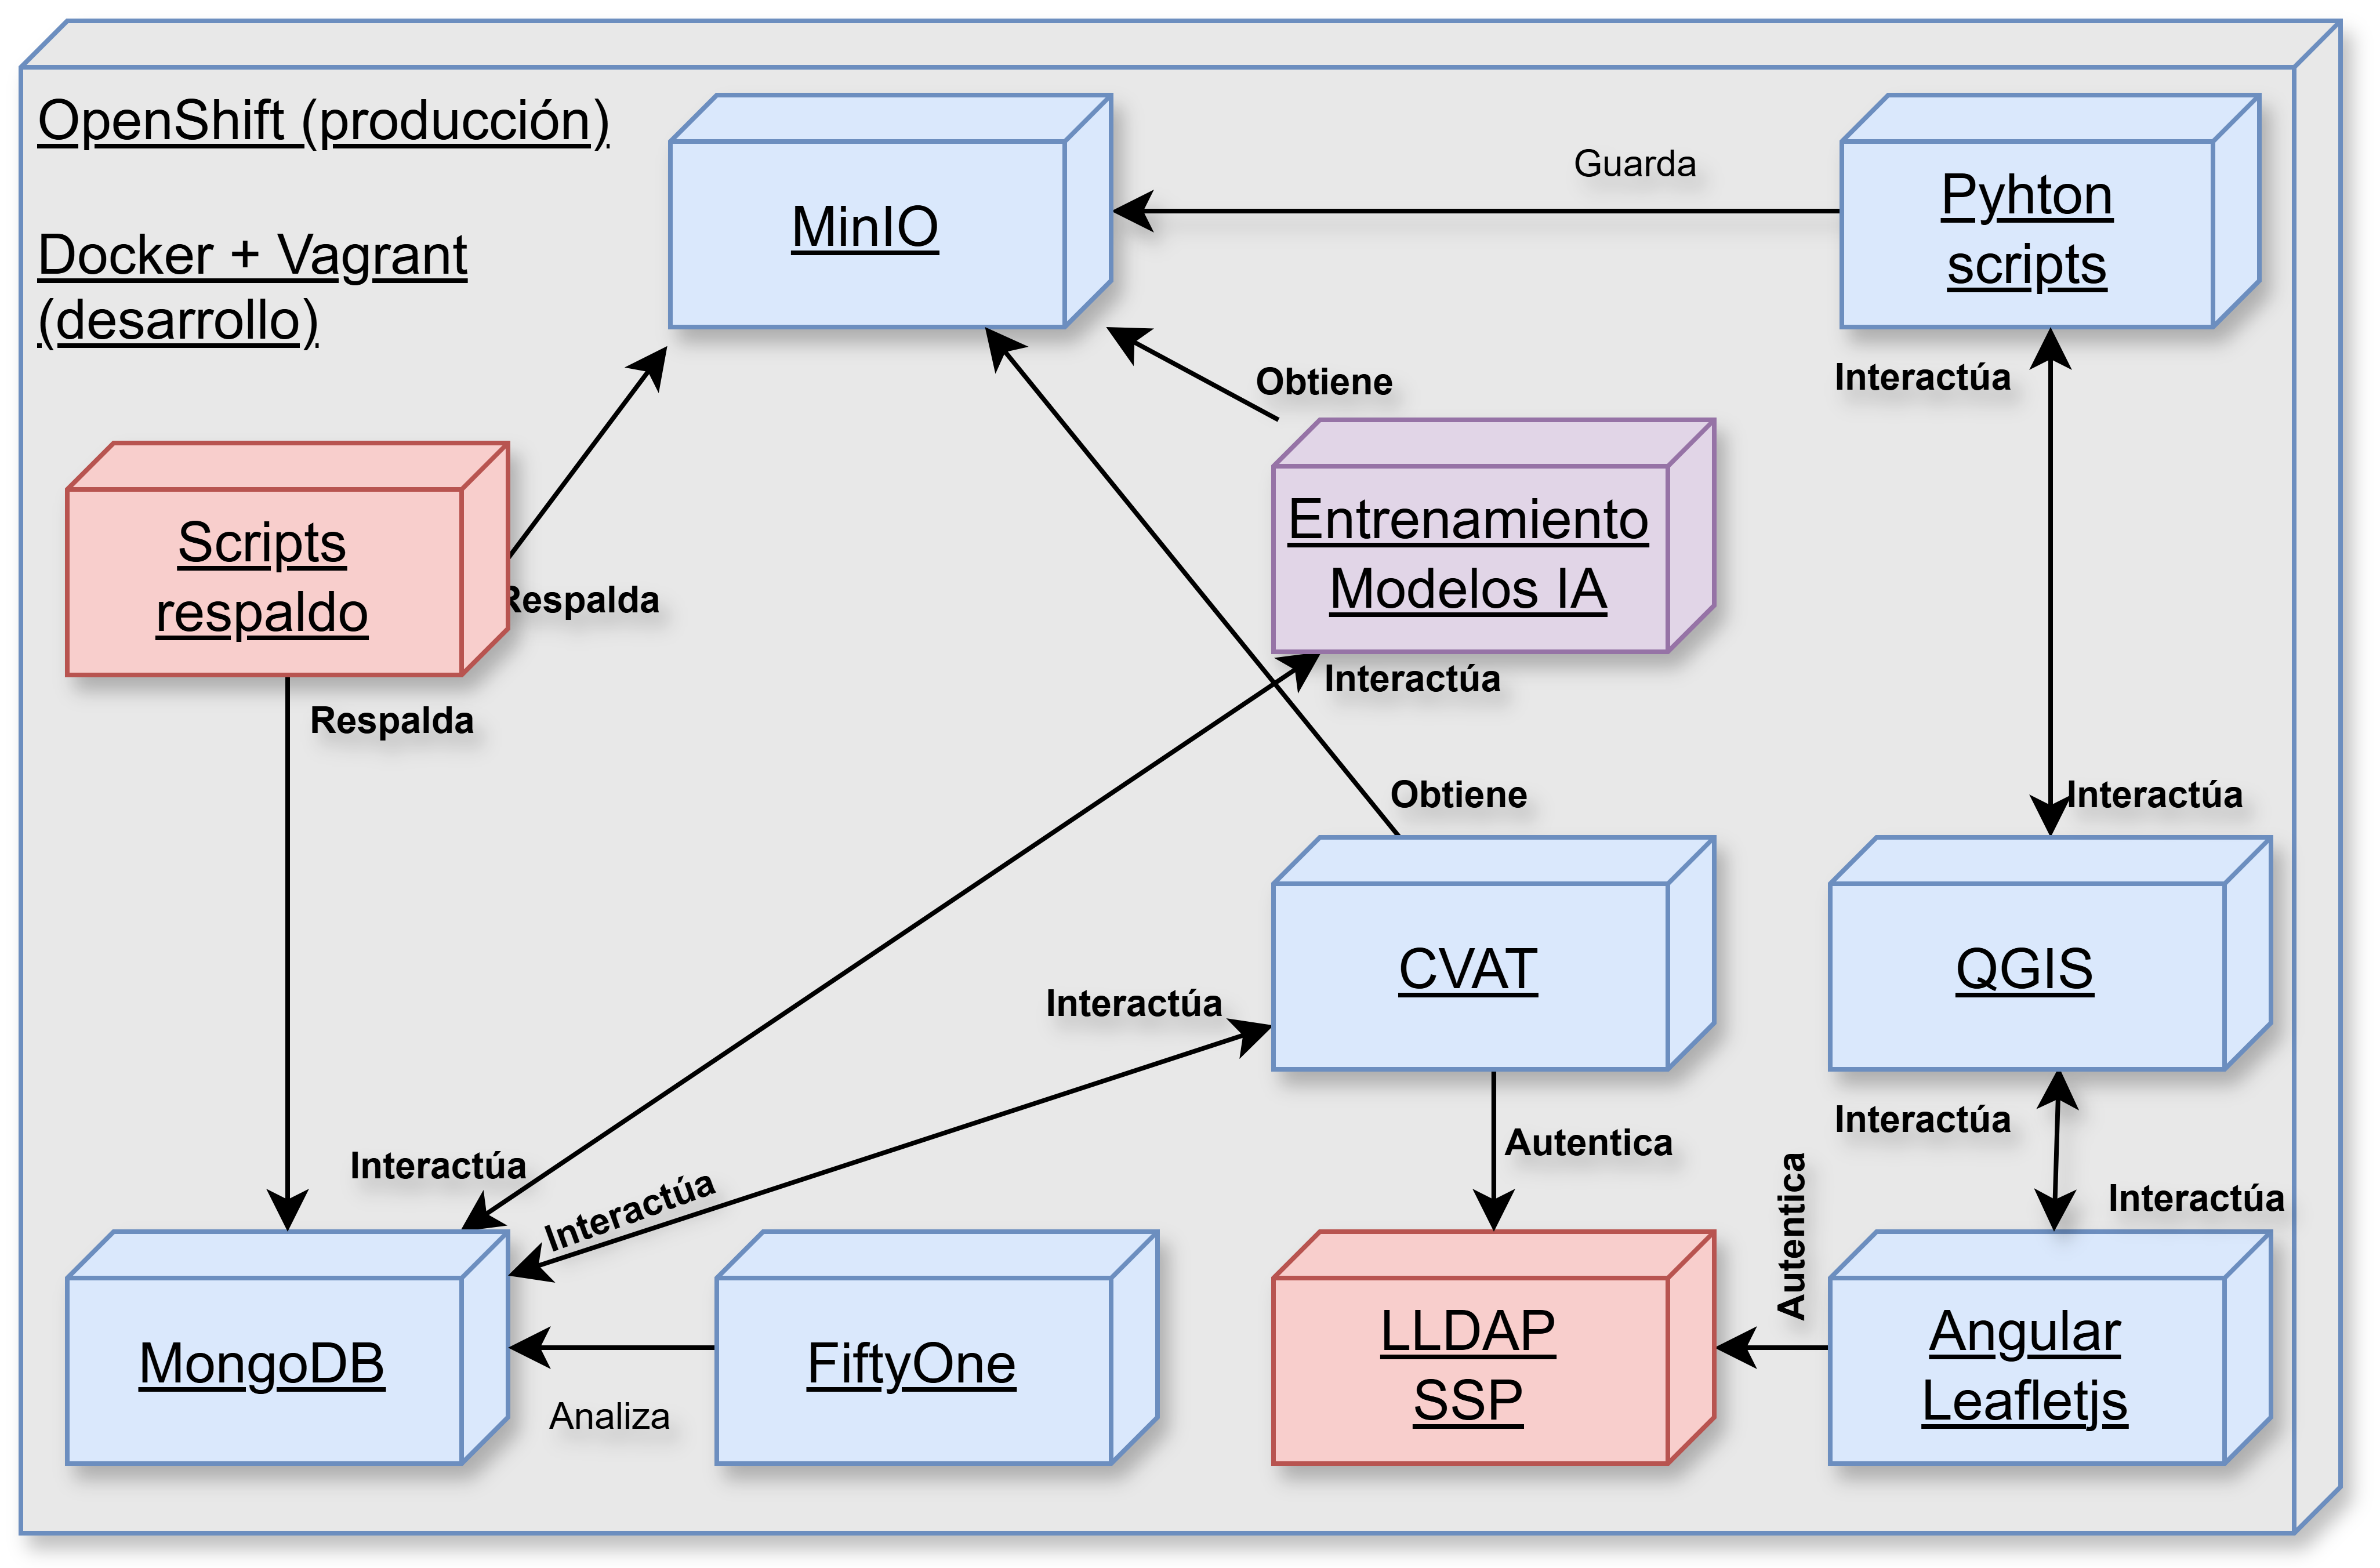
\includegraphics[scale=0.09]{./Figures/herramientas-plataforma.png}
  \caption{Diagrama de la plataforma de monitoreo.}
  \label{fig:infra-desarrollo}
\end{figure}

Otro usuario desarrollador puede tener el ambiente directamente desde su máquina, simplemente clonando el repositorio \citep{bruno_masoller_brunomaso1uba-ceia_nodate} mediante Git y luego importar el proyecto utilizando un IDE \citep{wikipedia_entorno_2025}. En este caso, se utilizó Visual Studio Code. Una vez importado el proyecto, la estructura de directorios emula cada módulo del proyecto de la siguiente manera:

% Ejemplos de código:

% \begin{lstlisting}[label=cod:vControl,caption=Estructura de directorios utilizada.]  % Start your code-block
%
%   desarrollo/
%     |-- cvat/
%
% \end{lstlisting}

% \usepackage{alltt}
% \begin{alltt}
%
%   desarrollo/
%   ├── cvat/
%
% \end{alltt}

\begin{lstlisting}[label=cod:vControl,caption=Estructura de directorios utilizada., literate={├}{{\textSFviii}}1 {─}{{\textSFx}}1 {└}{{\textSFii}}1 {│}{{\textSFxi}}1]  % Start your code-block

  desarrollo/
  ├── modulo-aplicaciones-web/
  │   ├── entrypoint/
  │   └── landing-page/
  ├── modulo-calidad-datos/
  │   └── fiftyone/
  ├── modulo-etiquetado-datos/
  │   └── cvat/
  ├── modulo-gestor-datos/
  │   └── mongo/
  ├── modulo-ia/
  │   ├── YoloV11/
  │   ├── Faster R-CNN/
  │   ├── ConvNeXt/
  │   ├── EfficientDet/
  │   └── DETR/
  ├── modulo-informacion-georreferenciada/
  │   └── QGIS/
  ├── modulo-mini-apps/
  │   └── webscrapping-SIG/
  ├── modulo-repositorio-objetos/
  │   └── MinIO/
  ├── modulo-respaldo/
  │   └── scripts/
  ├── modulo-seguridad/
  │   ├── SSP/
  │   └── LLDAP/
  ├── vagrant-scripts/
  ├── readme.md
  └── Vagrantfile

\end{lstlisting}

Esta estructura permite que luego se puedan sustituir estas herramientas por su análogo en la infraestructura de la IM. Por ejemplo, LLDAP puede ser sustituido por WSO2.

En ingeniería de software es importante asegurar la reproducibilidad de los ambientes de trabajo. Una de las herramientas utilizadas para asegurar esto es Docker, que habilita crear contenedores que encapsulan una aplicación y sus dependencias. Esto asegura un entorno de ejecución uniforme y reproducible en diferentes sistemas. Para la orquestación de múltiples contenedores se utilizó Docker Compose, que brinda una infraestructura en entornos complejos en donde interactúan varias aplicaciones.

Cada directorio tiene su propio archivo de Docker Compose (\lstinline[language=sh]|docker-compose.yml|) que habilita el despliegue de las herramientas del módulo. Esto, además de las ventajas mencionadas anteriormente en la sección \ref{sec:arquitectura}, también permite que cada componente pueda ser desarrollado y probado de manera independiente (con sus debidos \textit{stubs} \citep{wikipedia_talon_2025} o \textit{mocks} \citep{wikipedia_objeto_2024}), lo que reduce el Lead Time \citep{wikipedia_lead_2025}. Estos archivos de configuración pueden ser adaptados a distintas situaciones. Por ejemplo, el archivo \lstinline[language=sh]|docker-compose.yml| de MinIO fue adaptado para que, si no existe el \textit{bucket} llamado "picudo-rojo-bucket", se cree automáticamente.

Asimismo cada módulo tiene sus variables de entorno definidos como archivos .env su directorio raíz. Esto permite separar la configuración de los distintos ambientes para cada módulo. En este sentido, concede la fácil transición entre el ambiente de desarrollo y el ambiente de producción. Cuando se ejecute en el ambiente de producción, estos archivos de configuración se pueden migrar a ConfigMaps \citep{red_hat_chapter_nodate} y Secrets \citep{red_hat_chapter_nodate-1} de OpenShift, que permiten gestionar la configuración de los contenedores de manera segura y eficiente. Esto asegura que la información sensible, como contraseñas o claves de acceso, no se exponga en el código fuente.

Aunque Docker permite crear contenedores que emulan el ambiente de producción, esto no es suficiente para asegurar la reproducibilidad de este dominio en el entorno de desarrollo. Esto se debe a que Docker se ejecuta sobre una plataforma, que puede ser diferente en cada máquina. Por lo tanto, es necesario utilizar una herramienta que permita crear y gestionar la infraestructura de soporte de manera uniforme y reproducible. Para esto se utilizó Vagrant.

Vagrant concede la habilidad de crear una o varias máquinas virtuales (VM, del inglés \textit{virtual machine}) que emulan una plataforma objetivo, en este caso, se podría crear una VM con la misma versión del sistema operativo que se utiliza en el ambiente real (RHEL \citep{red_hat_sistema_nodate}). Se maneja con un archivo de configuración llamado Vagrantfile que brinda la posibilidad de realizar la definición de la configuración de la máquina virtual como \textit{infrastructure as a code}. Esto implica definir parámetros como la cantidad de memoria, el sistema operativo o las aplicaciones a instalar. Se puede utilizar una imagen de un sistema operativo ya configurado o crear una desde cero. En este caso se utilizó una imagen de Ubuntu 24.04 LTS \citep{progress_chefs_bento_bentoubuntu-2404_nodate}, del repositorio oficial de Vagrant \citep{hashicorp_hashicorp_nodate}, que incluye la mayoría de las herramientas necesarias para el desarrollo y despliegue del sistema. Esta imagen se puede utilizar en cualquier máquina que tenga instalado Vagrant y VirtualBox \citep{wikipedia_virtualbox_2025} (también se puede utilizar otro software de virtualización, como lo es Hyper-V \citep{meaghanlewis_informacion_2025} o VMWare \citep{wikipedia_vmware_2025}), por lo que si otro desarrollador se incorpora al proyecto, al utilizar la misma imagen puede tener el mismo ambiente de desarrollo. Esto asegura que el sistema funcione de la misma manera en diferentes máquinas y evita problemas de compatibilidad entre diferentes versiones de software.

Asimismo, Vagrant también permite aprovisionar \textit{scripts} de configuración a las máquinas virtuales. Estos pueden ejecutarse al iniciar estas máquinas, lo que permite instalar y configurar las aplicaciones necesarias para poner el funcionamiento el sistema. En este caso, se utilizaron cuatro scripts de aprovisionamiento:

\begin{lstlisting}[label=cod:dd,caption=Scripts de vagrant utilizados., literate={├}{{\textSFviii}}1 {─}{{\textSFx}}1 {└}{{\textSFii}}1 {│}{{\textSFxi}}1]  % Start your code-block

  vagrant-scripts/
  ├── 01-setup-network.sh
  ├── 02-install-dependencies.sh
  ├── 03-configure-firewall.sh
  └── 04-start-dev-services.sh

\end{lstlisting}

En donde el último se encarga de iniciar los servicios dentro de cada módulo (usualmente se ejecuta mediante un script de shell el comando \lstinline[language=sh]|docker compose up|).

Una vez que se ejecuta el comando \lstinline[language=sh]|vagrant up|, se crea una máquina virtual (si ya no fue creada), se ejecutan los scripts de aprovisionamiento, lo que resulta en el ambiente de desarrollo listo para utilizarse.

Entre los servicios que se inician se encuentran:

\begin{itemize}
  \item MongoDB: implementa la base de datos que permite almacenar metadatos de las imágenes ortorectificadas y los resultados de los modelos.
  \item MinIO: almacena las imágenes generadas por los drones y aviones.
  \item CVAT: se utiliza para etiquetar las imágenes almacenadas en el repositorio de objetos.
  \item FiftyOne: herramienta de análisis, organización, visualización y generación de informes sobre los datos.
  \item LLDAP: herramienta de gestión de usuarios y permisos, utilizada para administrar la seguridad del sistema.
  \item LDAP \textit{Self Service Password}: autoservicio de contraseñas (permite que los usuarios gestionen sus credenciales)
  \item \textit{Landing Page}: conjunto de herramientas basadas en tecnologías de desarrollo web (HTML, CSS, Javascript) que brindan información sobre el proyecto. Es la cara visible del sistema desde internet.
  \item Mini-apps: scripts que ejecutan varias tareas, como por ejemplo, obtener las imágenes desde el SIG de la IM.
  \item \textit{Entrypoint}: proxy reverso que expone el ambiente de desarrollo a internet o intranet para su fácil acceso.
\end{itemize}

% Poner un esquema de flujo (caso de uso) de la plataforma, mostrando los módulos y su interacción.
% Hablar un poco más sobre cada módulo y como se desliega.
% Mostrar alguna imagen del acceso desde internet a la plataforma, como por ejemplo el acceso a la landing page o al sistema de etiquetado de imágenes.
% Hablar de los problemas encontrados durante el despliege de la plataforma. Porque se eligió cada herramienta. Hablar del tema de CVAT vs Label Studio.

%----------------------------------------------------------------------------------------
%	SECTION 3
%----------------------------------------------------------------------------------------

\section{Proceso de etiquetado de datos}
\label{sec:etiquetado}

% Hablar de los tipos de usuarios, las pruebas que se realizaron -de control, no en profundidad- y las jornadas de etiquetado.
% También como se midió el progreso. Hablar del enfoque que se tomó (recortar las imágenes).
% Mostrar algunos de los etiquetados finales.

%----------------------------------------------------------------------------------------
%	SECTION 4
%----------------------------------------------------------------------------------------

\section{Entrenamiento de los modelos}
\label{sec:entrenamiento}

% Hablar del proceso de entrenamiento de los modelos.

%----------------------------------------------------------------------------------------
%	SECTION 5
%----------------------------------------------------------------------------------------

\section{Despliegue de los modelos}
\label{sec:despliegue_modelos}

% Hablar del proceso de despliegue de los modelos.
% Hablar de la integración con el resto de la plataforma.
% Hablar de las herramientas utilizadas para el despliegue de los modelos.
% Hablar de los problemas encontrados y como se resolvieron.
